%!TEX TS-program = pdflatex
%!TEX encoding = UTF-8 Unicode

% Template borrowed from Jeff Erickson via Kyle Fox

\documentclass[11pt]{article}
\usepackage{jeffe,handout,graphicx}
\usepackage[utf8]{inputenc}		% Allow some non-ASCII Unicode in source
\usepackage{xcolor}
\usepackage{mdframed}
\usepackage{arydshln}
\usepackage[normalem]{ulem}
\usepackage{bigdelim}
\usepackage{listings}
\usepackage{tabularray}
\usepackage{endnotes}
\usepackage{soul}
\newcommand{\hlc}[2][yellow]{{%
    \colorlet{foo}{#1}%
    \sethlcolor{foo}\hl{#2}}%
}


\let\footnote=\endnote
\lstset{language=R,
    frame=single,
    numbers=left,
    numberstyle={\tiny \color{black}},
    numbersep=9pt}

\definecolor{codebackcolor}{rgb}{0.9, 0.9, 0.75}
\definecolor{codenumcolor}{rgb}{0.5, 0.5, 0.5}
\definecolor{codecommentcolor}{rgb}{0.75, 0.25, 0.1}
\definecolor{codekeywordcolor}{rgb}{0.25, 0.00, 0.50}
\definecolor{codestringcolor}{rgb}{0.125, 0.00, 0.50}


\lstdefinestyle{mystyle}{
    backgroundcolor=\color{codebackcolor},   
    commentstyle=\color{codecommentcolor},
    keywordstyle=\color{codekeywordcolor},
    numberstyle=\tiny\color{codenumcolor},
    stringstyle=\color{codestringcolor},
    basicstyle=\ttfamily\footnotesize,
    breakatwhitespace=false,         
    breaklines=true,                 
    captionpos=b,                    
    keepspaces=true,                 
    numbers=left,                    
    numbersep=5pt,                  
    showspaces=false,                
    showstringspaces=false,
    showtabs=false,                  
    tabsize=2
}

	        
	\newcommand{\hlta}[1]{\colorbox{yellow!35}{\(\displaystyle#1\)}}
	\newcommand{\hltb}[1]{\colorbox{red!20}{\(\displaystyle#1\)}}
	\newcommand{\hltc}[1]{\colorbox{blue!20}{\(\displaystyle#1\)}}
	\newcommand{\hltd}[1]{\colorbox{green!30}{\(\displaystyle#1\)}}

\lstset{style=mystyle}
% from https://tex.stackexchange.com/questions/169679/vdots-are-taller-than-the-rest-of-text
\makeatletter
\DeclareRobustCommand{\rvdots}{%
  \vbox{
    \baselineskip3\p@\lineskiplimit\z@
    \kern-\p@
    \hbox{.}\hbox{.}\hbox{.}
  }}
\makeatother

% =========================================================
%   Define common stuff for solution headers
% =========================================================
\Class{CS 6320}
\Semester{Fall 2021}
\Authors{2}
\AuthorOne{Ziyad Amir Dhuka}{zxd200000}
\AuthorTwo{James Amato}{jca120030}
%\Section{}
\begin{document}
\HomeworkHeader{}{}% homework number, problem number

\begin{center}\huge{Natural Language, Processed Unnaturally}\end{center}

Hello Ximeng! Please note that this is a very preliminary draft. We will certainly be updating this, but wanted to give you a preview.

\section{Problem Description}

Given a limited knowledge set, answer several questions pertaining to it.

The data is a portion of the Stanford Question Answering Dataset (SQuAD). It consists of 30 articles and over 2500 questions.  We were provided some data with which to develop our solutions. The solution will be tested with unseen questions pertaining to those 30 articles. Thus, in the test environment, preprocessed articles are able to be used.

\section{Proposed Solution}

Our solution really does a decent job with task 1 and 3, and has a thought-through-for-many-hours-but-still-nonfunctioning answerer for task 2. Currently, the best performing method uses a simple keyword search, with keywords broken into individual tokens.

We use established libraries and software for processing and storing NLP information from the articles. Each question is similarly processed. We hope to establish a good method for processing questions based on \texttt{Lasso}, 2000 \cite{lasso2000}. For finding keywords, 

\section{Full Implementation Details}

blah

\subsection{Programming Tools}

All work is performed in Python.

The relational database used is \texttt{solr} \cite{solr}. It is Java-based, open-source, enterprise-level, and developed by contributors to the Apache Software Foundation.

The NLP pipeline uses many tools. NLTK is used for tokenization and POS-tagging \cite{nltk}. It is used in conjunction with WordNet for lemmatization and finding synonyms \cite{wordnet}. Named entities and parse trees are established using spaCy \cite{spacy2}.

When reading sentence, the RAKE (Rapid Automatic Keyword Extraction) algorithm is used. It was described by Rose, et al. in 2010 \cite{rake1}. The library implemention by Sharma leverages the strengths of nltk \cite{rake2}.


\subsection{Architectural Diagram}

[Architectural Diagram to be developed]

\subsection{Results and Error Analysis}

As development proceeded we found the need to determine when correct articles are found. Our analysis simply counts instances of the correct answer in the target sentence. The first system we built was meant to deliberately get things wrong, and simply returned the first result in the whole solr database, when searching for type:'sentence'. By default, this happened to be the first sentence in article 109, ``Bird migration is the regular seasonal movement, often north and south along a flyway, between breeding and wintering grounds.'' We counted number of times the article was correctly identified, and number of times the provided answer appeared in the sentence. Interestingly, because the terms ``north'' and ``south'' are answers to two unrelated questions, this method counted those as correct. Another question asked something similar, ``What is the most common direction of migration in autumn?''; the provided answer ``south'' appears in the provided answer. So we see it is an imperfect method.

Nevertheless, we proceed. We tried to make data-driven decisions. As such, when we found a reasonably good, albeit very simple answerer, we begain building tools for analysis. One such analysis looks at the solr score for a given result, and compares it when the answer is correct or incorrect, and when the article is determined correctly or incorrectly. We examined both the top score in those cases, and the deltas between scores. We did this analysis both on a small subset of questions (used for development) and the full set provided.

    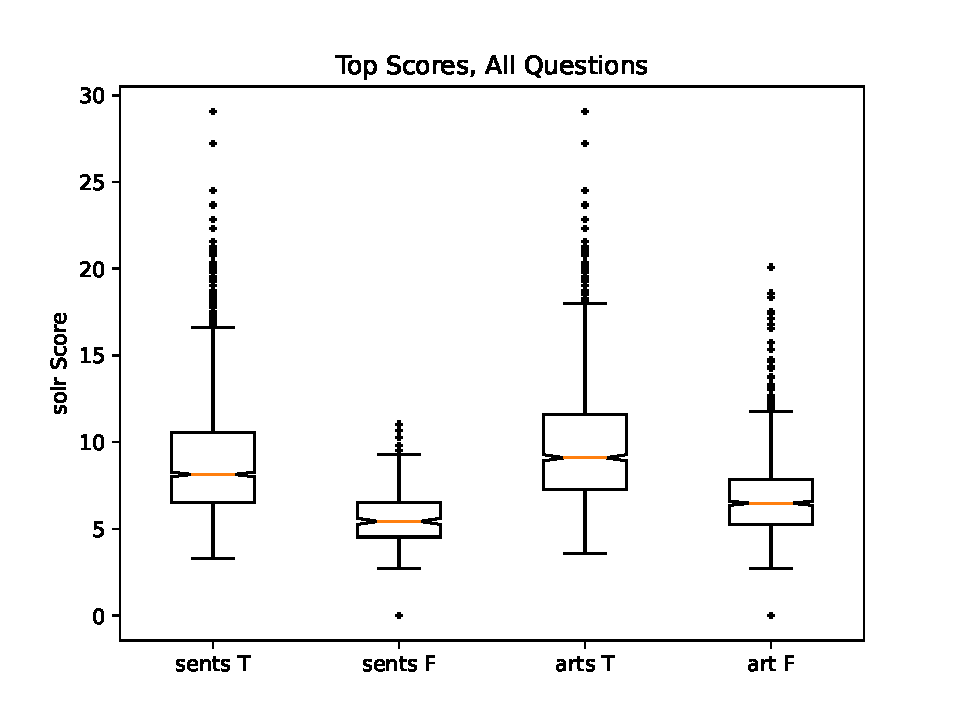
\includegraphics[trim={0 0 0 0},clip,scale=0.9]{fig/bt-all.pdf}
    
    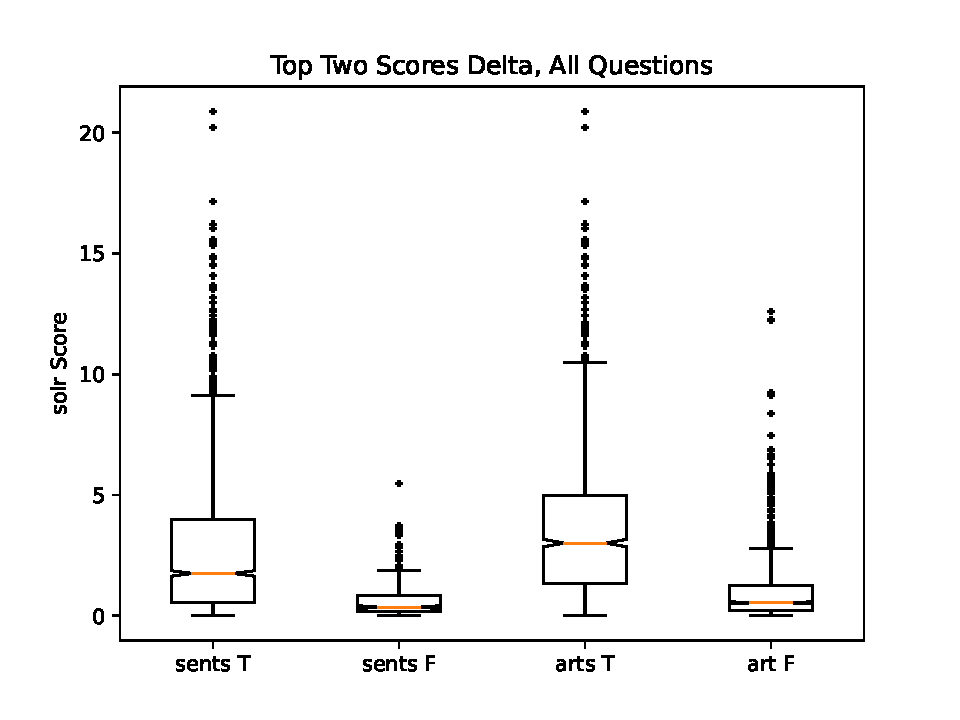
\includegraphics[trim={0 0 0 0},clip,scale=0.9]{fig/bd-all.pdf}

\subsection{Problems: Encountered and Resolved}

Initially, Jim had difficulty reading the data files into python, though Ziyad did not. The solution is always setting encoding='utf-8' when reading and writing files.

We built a BadAnswerer in hopes of getting the most improved award. This method simply returned the first sentence found in any article.  In the set of questions, 89 are for this article, so those are correct by default.

Interestingly, for BadAnswerer, the results were better than expected:

BadAnswerer: Of 2505 total questions, the correct article was found 89 times and the correct sentence was found 4 times.

Next method simply used RAKE keyword search. Of 2505 questions, got 1453 correct articles and 769 correct sentences.

KeywordAnswerer: Of 2505 total questions, the correct article was found 1453 times and the correct sentence was found 769 times.

Next method - broke RAKE keywords into component pieces. For instance, from the question: "On what did Skousen analyze ink and pencil remnants?" we previously found only 2 compound keywords ("skousen analyze ink" "pencil remnants"); now we find 5 ("skousen" "analyze" "ink" "pencil" "remnants")
Of 2505 total questions, the correct article was found 2206 times and the correct sentence was found 1380 times. (55\%)

Next method - blacklisting just two words ("one", "type"), which seem to be particular to questions, did not improve results.

While preparing to add NE utiliation, explored how question words are used. There is a list of questions, below, with multiple question words in a single question. Need to use better system (POS tagging? syntatic analysis?)

Some difficulty when trying to find meronyms and holonyms... because it's not quite as simple as that. More hours than I'm proud to admit were spent debugging, when in fact the proper solution is that wordNet breaks meronyms and holonyms into substance and part types.

\subsection{Pending Issues}

We are trying to apply scipy statistics to the score results, but get ridiculous and plainly incorrect p-values and confidence intervals (overestimating precision).

\subsection{Potential Improvements}

Time management skills, for real, am I right?!

Further work would employ more of the techniques found in \texttt{Falcon}, 2000 \cite{falcon2000}.

\bibliography{my}{}
\bibliographystyle{plain}

\end{document}